\subsection{General}
\acp{rnn} allow for cycles in the connectivity graph. These cycles allow information to persist in the network for some time (state) and provide a fading memory. This makes \acp{rnn} extremely powerful at processing sequences. \b{\acp{rnn} are Turing-complete and can represent dynamical systems rather than function mappings.}\\
There are several ways to use \acp{rnn}:
\begin{itemize}
    \item \b{One-to-many:} Image caption generation.
    \item \b{Many-to-one:} Giving a numerical score to a given review.
    \item \b{Many-to-many:} Video frame classification, language translation.
\end{itemize}

\subsection{Design Patterns}
\acp{rnn} produce outputs at every step \f{t}, with recurrent connections between hidden units. The unfolded network can be seen in the figure below. \acp{rnn} are trained with \ac{bptt}, which is backpropagation with weight sharing over the unrolled computational graph.\\
The forward pass is defined the following:
\cf{h^{(t)} = \tanh(Wh^{(t-1)}+Ux^{(t)} + b)}
\cf{\hat{y}^{(t)}=\text{softmax}(o^{(t)})=\text{softmax}(c+Vh^{(t)}),}
where \f{W,U,V} are shared weight matrices of the hidden units and \f{b,c} are shared bias vectors for the hidden states and outputs respectively.\\[0.5em]

\begin{figure}[ht]
    \centering
    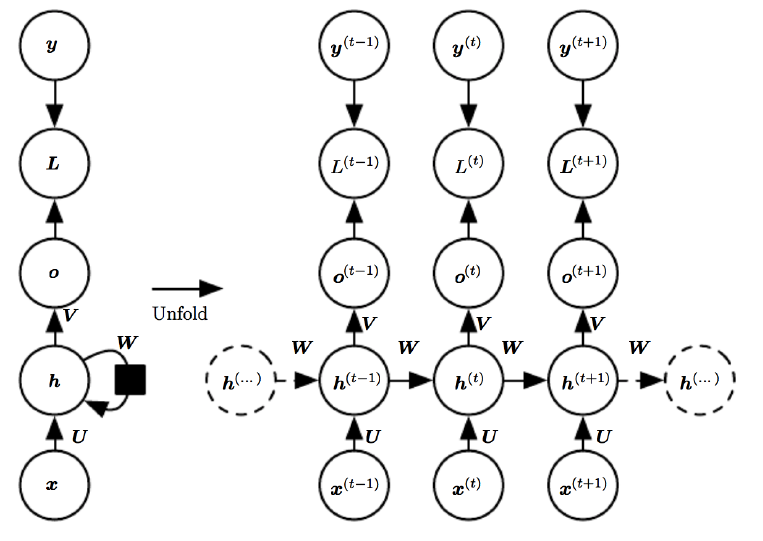
\includegraphics[width=0.5\textwidth]{rnn.png}
\end{figure}


An alternative to having the recurrent connections between the hidden units, is having them go \b{from the output to the successive hidden unit}. Even though this is potentially less powerful, it has the advantage that it can be trained with \b{teacher forcing}.\\
Here, during training time, the hidden layers are fed with the true label of the previous step instead of the models own prediction. This enables the model to learn from the data directly, but it approximates based on the predictions during test time which makes it likely to accumulate errors over time.

\subsection{Miscellaneous Architectures}
\begin{enumerate}
    \item \b{Many-to-One:} Recurrent connections etween hidden units, output only at last step (BPTT).
    \item \b{One-to-Many:} Mapping static input into distribution over sequences of \f{y}. Outputs at every step.
    \item \b{Many-to-Many:} Mapping variable length sequence of inputs into distribution over sequences of \f{y}. Can be combined with teacher forcing and \ac{bptt}.
\end{enumerate}

Additional architectures: \b{Bidirectional \ac{rnn}} with two directional hidden states can use information from both past and future. Since it requires future information, it cannot be used for online tasks. \b{Encoder-Decoder seq.-to-seq.} architecture are used when the length of inputs and outputs are different, such as for translation.

\subsection{Problems during Training}
Although RNNs have powerful non-linear processing due to the repeating application of the same function, it also induces some problems. Typical problems are gradient vanishing and explosion. The solution for the explosion is gradient clipping and that for the vanishing is the LSTM.

\subsection{Truncated BPTT}
BPTT is expensive and possibly unstable. Furthermore it can lead to vanishing/exploding gradients. The solution is to use truncated BPTT, which truncates gradients after fixed intervals (often aligned with batch-size). Requires sequential data loading. 

\subsection{\ac{lstm}}
The LSTM was introduced to address the vanishing gradient problem. Its architecture consists of special memory cells with \b{forget, input} and \b{outpus gates}. By now the LSTM has become the standard RNN model in many applications.\\[0.3em]

\begin{figure}[ht]
    \centering
    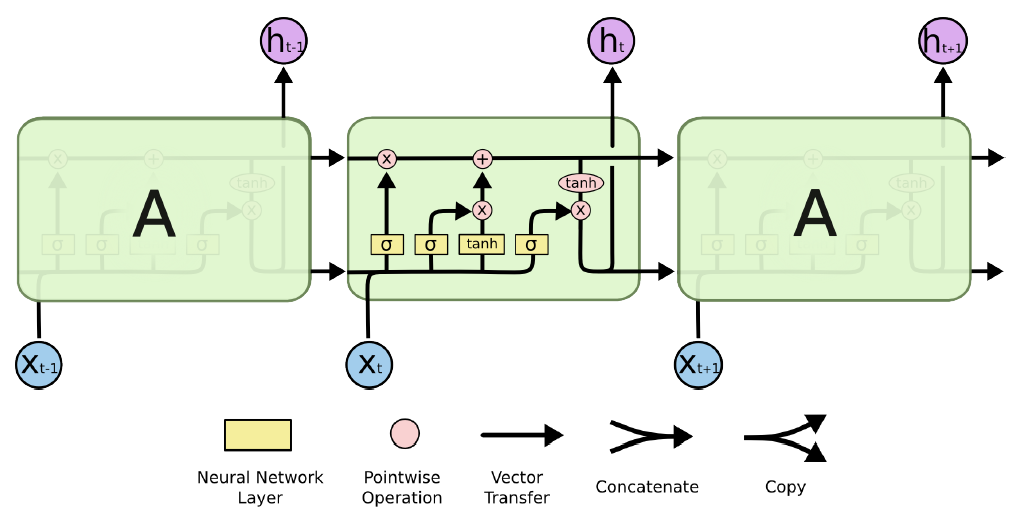
\includegraphics[width=0.7\textwidth]{lstm.png}
\end{figure}

Since this model has a self-loop of inner state \f{C} without any activations, the gradient with respect to \f{C} does not vanish nearly as RNNs do. The forget gate decays less important features from the past and maintain important features. The input gate takes two vectors \f{i_t} and \f{\tilde{c_t}} and controls how much new information we should store and in which direction we should change the state. The output gate controls which features to use. The advantages of LSTM are that it can selectively forget and remember features and each parameter of LSTM already have their meanings.